\documentclass[12pt,letterpaper]{article}

% --- Paquetes Requeridos ---
\usepackage[utf8]{inputenc}
\usepackage[spanish,es-tabla]{babel}
\usepackage[margin=2.5cm]{geometry}
\usepackage{graphicx}
\usepackage{float}
\usepackage{titlesec}
\usepackage{setspace}
\usepackage{hyperref}
\usepackage{booktabs}
\usepackage{caption}
\usepackage{enumitem}
\usepackage{listings}
\usepackage{xcolor}

% --- Configuración de Párrafo ---
\onehalfspacing
\setlength{\parindent}{0pt}
\setlength{\parskip}{1em}

% --- Rutas de búsqueda de imágenes ---
% Permite compilar tanto desde Documentos/Entregables/ como con todas las
% imágenes en una sola carpeta plana.
\graphicspath{{./}{../Evidencia/}{Evidencia/}{imagenes/}}

% --- Configuración de listings ---
\lstset{
    basicstyle=\ttfamily\footnotesize,
    breaklines=true,
    frame=single,
    captionpos=b,
    showstringspaces=false
}

% --- Inicio del Documento ---
\begin{document}

% --- PORTADA ---
\begin{titlepage}
    \centering

    {\Large \textbf{UNIVERSIDAD SANTO TOMÁS}} \\[1cm]

    {\Large \textbf{Sistema colaborativo de robots móviles para asistencia de orientación en entornos interiores con múltiples pisos}} \\[2cm]

    {\large \textbf{Realizado por:}} \\
    {\large Santiago Hernández Ávila} \\
    {\large Jonny Alejandro Mejía León} \\[1cm]

    \begin{figure}[H]
        \centering
        \includegraphics[width=0.6\textwidth]{Logos Uni.png}
        \label{Logo Universidad Santo Tomas y facultad de ingenieria electronica}
    \end{figure}

    \vfill

    {\large \textbf{Informe de Avance --- Semana 18}} \\
    {\large Fase 5: Integración del sistema y realización de pruebas --- Cierre del hito H1 y construcción del entorno de evaluación de dos niveles} \\[1.5cm]

    \textbf{Dirigido por:} \\
    Ing. Armando Mateus Rojas, Msc. \\
    Ing. Nestor Ivan Ospina, Msc. \\
    Ing. Oscar Mauricio Gélvez Lizarazo, Msc. \\[1.0cm]

    \vfill

    {\large GED (Grupo de Estudio y Desarrollo en Robótica)} \\
    {\large Facultad de Ingeniería Electrónica} \\
    {\large División de Ingenierías} \\
    {\large Bogotá, agosto de 2026}
\end{titlepage}

% --- CONTENIDO ---

\section{Introducción}

El presente informe documenta el avance correspondiente a la \textbf{Semana 18} del cronograma de actividades, dentro de la \textbf{Fase 5 (Integración del sistema y realización de pruebas)}.

La semana estuvo dedicada a completar las dos condiciones que habilitan la totalidad del desarrollo restante del proyecto. La primera es el \textbf{hito H1}: que dos agentes robóticos puedan operar de forma autónoma y simultánea sin que el mando de uno alcance al otro. La segunda es el \textbf{hito H2b}: que exista un entorno de evaluación con dos niveles verticales reales, sin el cual la métrica principal del objetivo específico 4 ---la continuidad del servicio entre niveles--- no se puede medir, únicamente declarar.

Ambos hitos quedaron cerrados con verificación instrumentada. Adicionalmente se detectó y corrigió un defecto en el mapa de navegación que habría comprometido cualquier métrica obtenida sobre él, y se consolidó la reproducibilidad del entorno de desarrollo.

Este informe presta atención particular, en la Sección \ref{sec:aporte}, a la relación entre cada actividad ejecutada y el objetivo específico al que contribuye. La Semana 18 produjo principalmente \emph{habilitadores}: componentes cuyo valor no se mide en avance porcentual propio sino en el trabajo que desbloquean. Se consideró preferible hacer explícita esa relación antes que presentar un avance agregado que no reflejaría la naturaleza del trabajo realizado.

\section{Objetivos de la Semana}

\begin{itemize}
    \item Cerrar el hito \textbf{H1}: dos agentes robóticos con pila de navegación completa, cada uno bajo su propio espacio de nombres, alcanzando objetivos de forma simultánea y con aislamiento de mando demostrado.
    \item Construir el \textbf{entorno de evaluación de dos niveles} y demostrar navegación autónoma sobre el nivel superior.
    \item Ejecutar el \textbf{diagnóstico acotado de hardware} sobre los vehículos físicos.
    \item Emitir el entregable de la Semana 17 y la \textit{Actividad 1 --- Corte 1} para revisión de los directores.
    \item Construir la matriz de requisitos que relaciona requisitos funcionales, objetivos específicos y pruebas de verificación.
\end{itemize}

De estos cinco objetivos se cumplieron tres. El diagnóstico de hardware y la matriz de requisitos no se ejecutaron y se trasladan a la Semana 19; las razones y sus consecuencias se exponen en la Sección \ref{sec:cronograma}.

\section{Cierre del hito H1: dos agentes autónomos aislados}

\subsection{Topología de simulación: un simulador por vehículo}

La primera aproximación consistió en instanciar los dos vehículos dentro de un mismo proceso simulador. Se comprobó que \textbf{no es viable}: la capa de integración entre Gazebo y ROS 2 en la distribución Humble aplica a todos los complementos cargados el espacio de nombres del \emph{primer} modelo instanciado. En consecuencia, los dos vehículos compartían un único tópico de comandos de velocidad, un único tópico de odometría y un único tópico de LiDAR, y la prueba de aislamiento no podía siquiera formularse.

La solución adoptada no es una corrección del código sino un cambio de topología: \textbf{un proceso simulador por vehículo}, cada uno con su propio identificador de dominio ROS y su propia dirección de servidor de simulación. Esta decisión no constituye un rodeo para esquivar una limitación de la herramienta, sino la traducción fiel del alcance del anteproyecto, que establece que cada robot opera de forma dedicada en un nivel específico y que la coordinación ocurre a través de un servidor. Además reproduce uno a uno el despliegue físico previsto, en el cual cada vehículo dispone de su propia unidad de cómputo.

Se verificó que la topología es sostenible en el equipo disponible. Con dos simulaciones activas de forma simultánea, el factor de tiempo real se mantuvo en 0,998 en ambas instancias, y durante la navegación con las dos pilas de Nav2 en ejecución se mantuvo en 0,996. Esta comprobación es una condición necesaria del objetivo específico 4: si la simulación no corriera a tiempo real, las métricas temporales quedarían contaminadas por falta de cómputo.

\begin{table}[H]
    \centering
    \small
    \caption{Consumo de recursos con dos simulaciones simultáneas.}
    \label{tab:recursos}
    \begin{tabular}{@{}lccc@{}}
        \toprule
        \textbf{Escenario} & \textbf{Factor de tiempo real} & \textbf{Hilos de 12} & \textbf{Uso de GPU} \\ \midrule
        Una simulación con visor       & 0,999 & ---  & ---    \\
        Dos simulaciones con visor     & 0,998 / 0,998 & 4,7 & 67 \% \\
        Dos simulaciones sin visor     & ---   & 4,6  & 22 \% \\ \bottomrule
    \end{tabular}
\end{table}

El cuello de botella identificado no es el procesador sino la memoria de la tarjeta gráfica integrada. Se establece en consecuencia que la operación por defecto durante las campañas experimentales sea sin visor gráfico, lo que reduce el uso de la GPU del 67 \% al 22 \%.

\subsection{Navegación y localización bajo espacio de nombres}

La pila de navegación no admitía espacios de nombres. Al lanzarla con prefijo, el mapa de costos global fallaba de forma repetida porque buscaba marcos de referencia sin prefijar mientras el vehículo los publicaba prefijados.

Se desarrolló un archivo de lanzamiento de localización propio, en sustitución del que provee la distribución de Nav2. La razón es que este último falla \textbf{sin producir ningún mensaje de error}, por dos motivos independientes:

\begin{enumerate}[leftmargin=*]
    \item Sus nodos no reciben el espacio de nombres. El argumento correspondiente se emplea únicamente para anidar el archivo de parámetros; quien aplica el espacio de nombres a los nodos es un componente superior que en esta topología no se utiliza. El resultado es que los nodos arrancan en la raíz, leyendo un archivo de parámetros anidado bajo una clave que no les corresponde, y por tanto \textbf{operan con los valores por defecto compilados en el código}.
    \item Remapea el tópico de transformadas de forma fija. Bajo espacio de nombres, eso envía la transformada de localización a un tópico distinto del que emplean el publicador de estado del robot y el simulador, con lo cual el árbol de transformadas queda partido en dos.
\end{enumerate}

Se registran dos precauciones de configuración cuyo incumplimiento produce fallos silenciosos, y que se documentan por su valor para el resto del proyecto:

\begin{itemize}
    \item \textbf{El anidamiento del archivo de parámetros es obligatorio.} El archivo contiene claves de primer nivel que solo corresponden a nodos sin prefijar. Sin anidarlas bajo la clave del espacio de nombres, los nodos arrancan con los valores por defecto del código, en silencio.
    \item \textbf{Las sustituciones de parámetros deben expresarse por ruta completa y no por clave suelta.} La clave que designa el marco global aparece dos veces en el archivo con valores distintos: uno para el mapa de costos global y otro para el local. Sustituirla por clave suelta igualaría ambos valores y rompería el mapa de costos local sin emitir ningún error.
\end{itemize}

La aplicación del espacio de nombres se realizó bajo un criterio metodológico explícito, heredado de la semana anterior: \textbf{cada cambio se introduce con un valor por defecto que reproduce el comportamiento previo, y se demuestra primero que no cambia nada}. Con espacio de nombres vacío se comparó parámetro a parámetro el archivo efectivo contra el archivo en disco: las únicas diferencias son las que el lanzamiento original ya introducía. Ningún marco de referencia cambia y ninguna clave se anida.

\subsection{Verificación del aislamiento de mando}

El resultado se verificó mediante cuatro evidencias independientes, \textbf{ninguna de las cuales se apoya en el desplazamiento observado} de los vehículos. Este criterio es deliberado: el desplazamiento es la evidencia más intuitiva y también la más frágil, porque depende de la lectura de odometría, que es precisamente donde se detectó un defecto abierto (Sección \ref{sec:abiertos}).

\begin{table}[H]
    \centering
    \small
    \caption{Evidencias de aislamiento entre los dos agentes.}
    \label{tab:aislamiento}
    \begin{tabular}{@{}p{5.2cm}p{8.3cm}@{}}
        \toprule
        \textbf{Evidencia} & \textbf{Resultado} \\ \midrule
        Inventario de tópicos por dominio & \textbf{62 tópicos en cada dominio y ninguno cruzado}: cero tópicos del segundo agente visibles desde el primero, y viceversa \\ \addlinespace
        Suscriptores del tópico de comando & Una \textbf{única} suscripción, la del complemento de tracción del propio vehículo. Los cuatro publicadores pertenecen a la pila de navegación del mismo agente \\ \addlinespace
        Procesos de simulación & Dos procesos independientes, con identificadores distintos \\ \addlinespace
        Comprobación visual & Al comandar el primer vehículo, el segundo permanece inmóvil en su propio visor \\ \bottomrule
    \end{tabular}
\end{table}

La primera evidencia es la de mayor peso porque constituye una \textbf{prueba de imposibilidad}: no se comprueba que un mensaje no haya cruzado, sino que no existe el canal por el cual podría hacerlo.

Complementariamente, se midió el desplazamiento real de ambos vehículos ante un objetivo de navegación enviado de forma simultánea. La medición se contrasta contra la odometría del simulador y no contra la estimación de localización, criterio adoptado por el proyecto y justificado en la Sección \ref{sec:mapa}.

\begin{table}[H]
    \centering
    \small
    \caption{Navegación simultánea de los dos agentes hacia un objetivo a 5,0 m.}
    \label{tab:navegacion}
    \begin{tabular}{@{}lccc@{}}
        \toprule
        \textbf{Agente} & \textbf{Recorrido real} & \textbf{Residuo} & \textbf{Resultado de la acción} \\ \midrule
        robot1 & 4,89 m & 11 cm & Objetivo alcanzado \\
        robot2 & 4,96 m & 4 cm  & Objetivo alcanzado \\ \bottomrule
    \end{tabular}
\end{table}

Se deja constancia del alcance exacto de lo demostrado: el aislamiento está garantizado por construcción, al existir dominios y simuladores separados. Estas pruebas verifican que la construcción es la que se cree, no descubren un aislamiento inesperado. Los dos vehículos no comparten espacio físico, lo cual es una limitación declarada del alcance y no un resultado del trabajo.

\subsection{Corrección de las referencias a los modelos geométricos}

Al preparar la evidencia visual se encontró que los doce eslabones del vehículo no se representaban en la herramienta de visualización. La causa no guardaba relación con el espacio de nombres: las referencias a los archivos de geometría estaban escritas sin el nombre del paquete que las contiene, de modo que el visualizador buscaba un paquete inexistente. Se corrigieron 26 apariciones.

La corrección \textbf{rompió la visualización en el simulador}, que resuelve la misma referencia por un mecanismo distinto. Se trata de una misma cadena de texto que debe satisfacer a dos resolvedores con reglas diferentes. La solución consistió en ampliar la ruta de búsqueda exportada por el paquete, de modo que ambas resoluciones sean válidas. El resultado se verificó visualmente en las dos herramientas de forma simultánea (Figura \ref{fig:rviz}).

Se registra una distinción operativa de valor diagnóstico: un modelo sin geometría visible \textbf{no es un modelo que no se cargó}. En el simulador el vehículo aparecía con sus siete eslabones, sus seis articulaciones y sus dos complementos cargados, pero sin geometría que dibujar. Confundir ambos casos habría orientado la investigación hacia un supuesto fallo del espacio de nombres.

\begin{figure}[H]
    \centering
    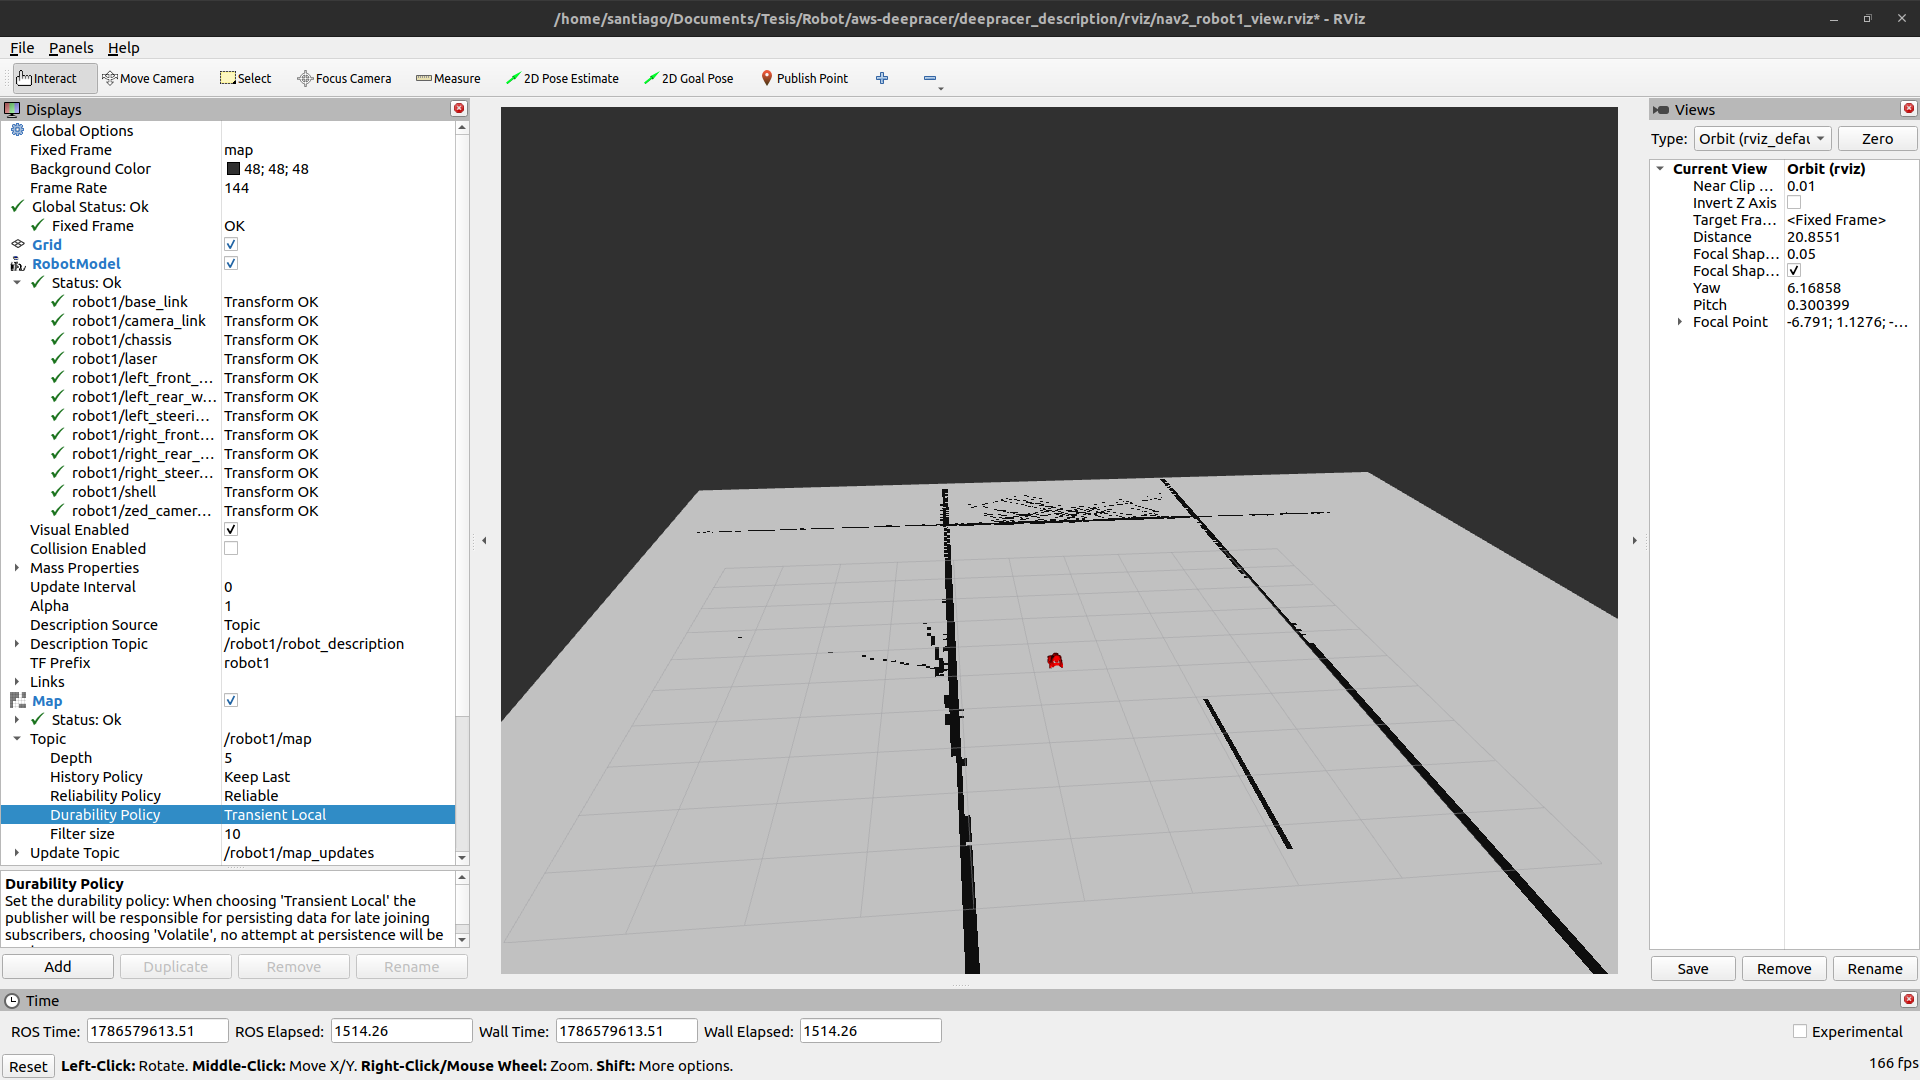
\includegraphics[width=0.85\textwidth]{S17_rviz_robot1_robotmodel.png}
    \caption{Modelo del vehículo representado correctamente en la herramienta de visualización, bajo el prefijo de marcos del primer agente.}
    \label{fig:rviz}
\end{figure}

\begin{figure}[H]
    \centering
    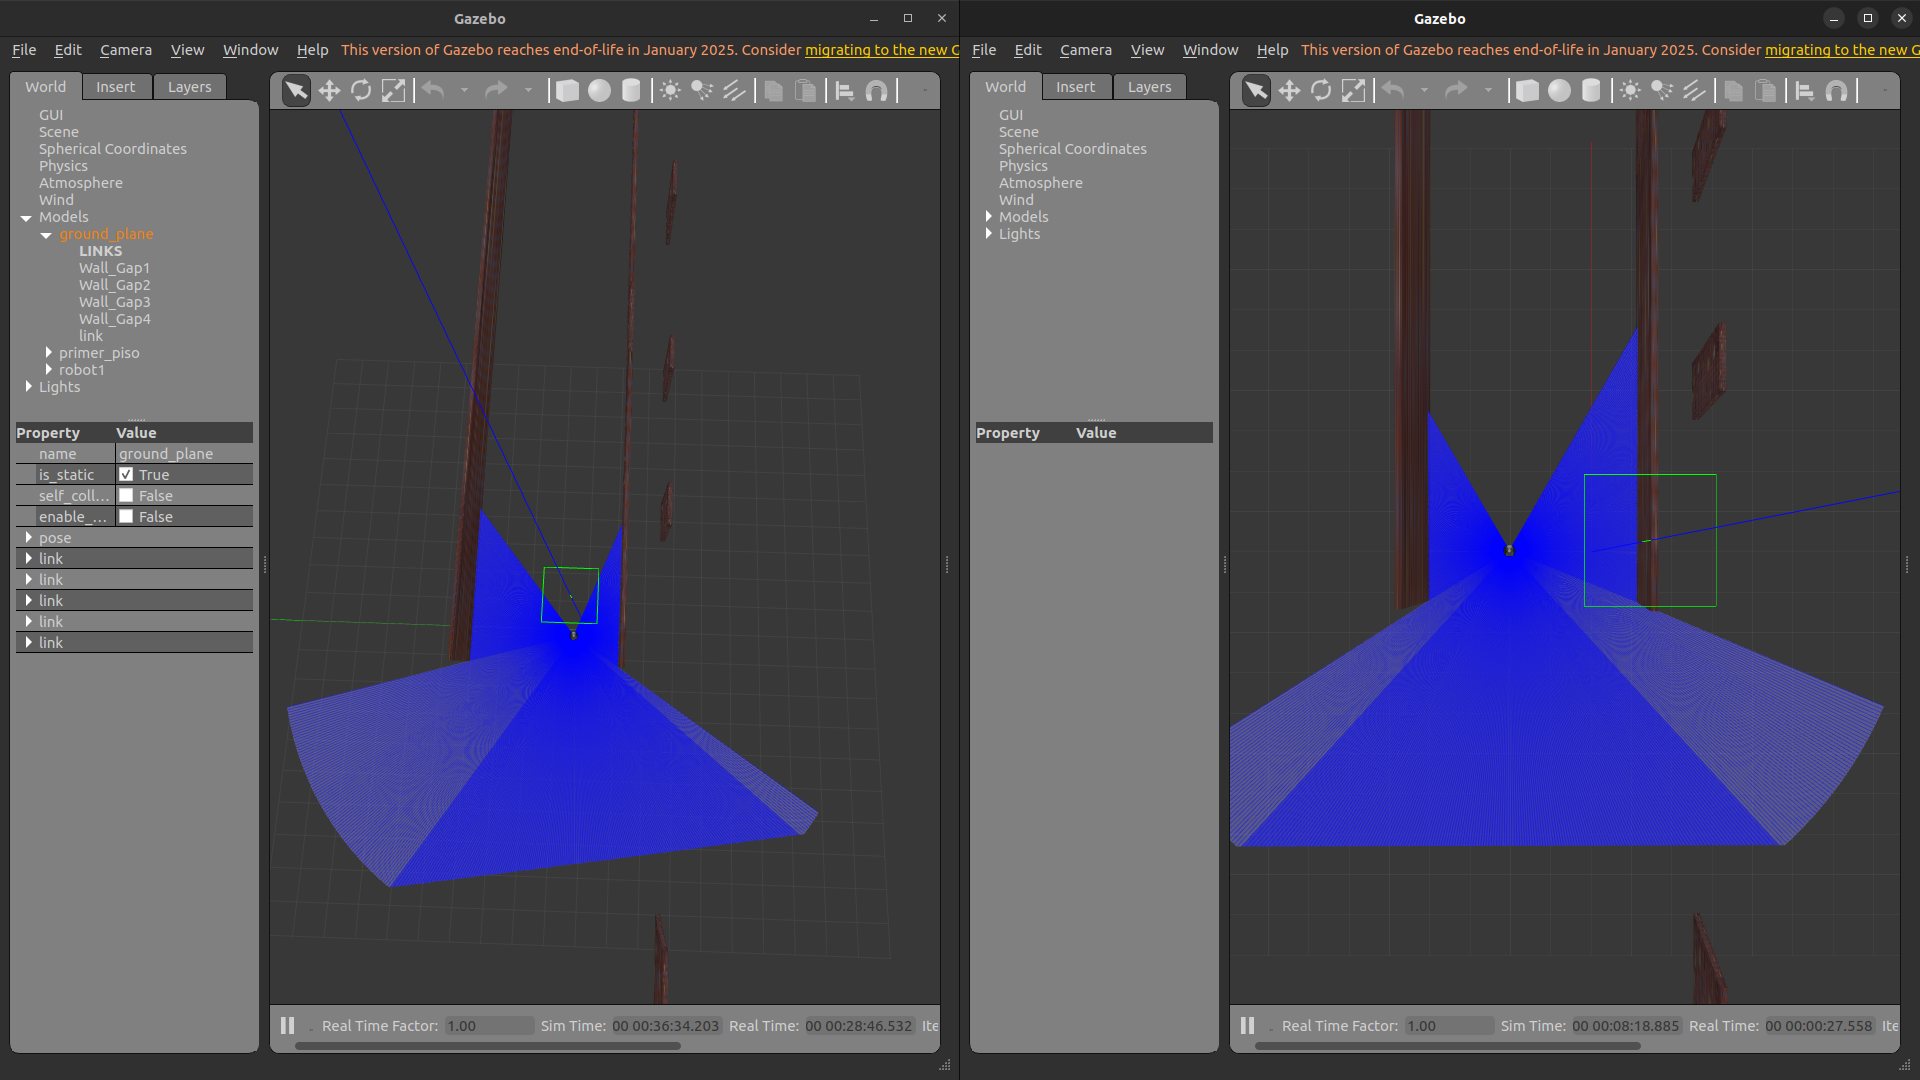
\includegraphics[width=0.95\textwidth]{S17_dos_gazebo_lado_a_lado.png}
    \caption{Dos procesos de simulación independientes ejecutándose de forma simultánea, cada uno con un vehículo.}
    \label{fig:dos_sim}
\end{figure}

\section{Entorno de evaluación de dos niveles}

\subsection{Motivación}

La cuarta métrica del objetivo específico 4 es la \textbf{continuidad del servicio entre niveles}. Constituye además la variable de respuesta principal de la pregunta de investigación formulada en el informe de la semana anterior. Sin un nivel superior navegable, esa métrica no admite medición: solo permite ser declarada.

\subsection{Extracción de la planta como modelo reutilizable}

La planta del primer piso se encontraba escrita en línea dentro del archivo de mundo, forma que impide instanciarla dos veces. Se extrajo a un modelo independiente y reutilizable.

La actividad partía de una premisa que resultó ser falsa. Un registro anterior del proyecto afirmaba que las poses declaradas en dos bloques distintos del archivo se contradecían en aproximadamente 21 m, lo que habría obligado a decidir cuál de las dos era correcta. Al verificarlo se comprobó que \textbf{no se contradicen}: unas son absolutas y las otras relativas al modelo. Restando la pose del modelo se recuperan exactamente las relativas en los doce muros, con residuos inferiores a 0,1 mm, que es el redondeo del propio archivo. Lo desplazado era el bloque completo, no la geometría.

Esta corrección tiene consecuencia directa sobre la validez del mapa: de esa supuesta discrepancia procedía la duda sobre si el mapa de navegación correspondía a la geometría simulada. Queda establecido que sí corresponde.

Como comprobación cruzada independiente, los muros del modelo extraído abarcan el intervalo de 1,24 m a 43,05 m en el eje longitudinal, mientras que el mapa vigente abarca de 1,20 m a 43,00 m. La coincidencia confirma que la extracción quedó ubicada donde el mapa ya la esperaba.

\subsection{Construcción del entorno}

El entorno se compone de dos instancias de la planta, situadas a 3,0 m de separación vertical, más una losa estática que sirve de piso al nivel superior, necesaria porque el plano de tierra del simulador solo existe en la cota cero. La losa se centró de modo que cubra la totalidad de la planta; una propuesta inicial la habría dejado 8 m corta respecto del extremo de los muros.

\begin{figure}[H]
    \centering
    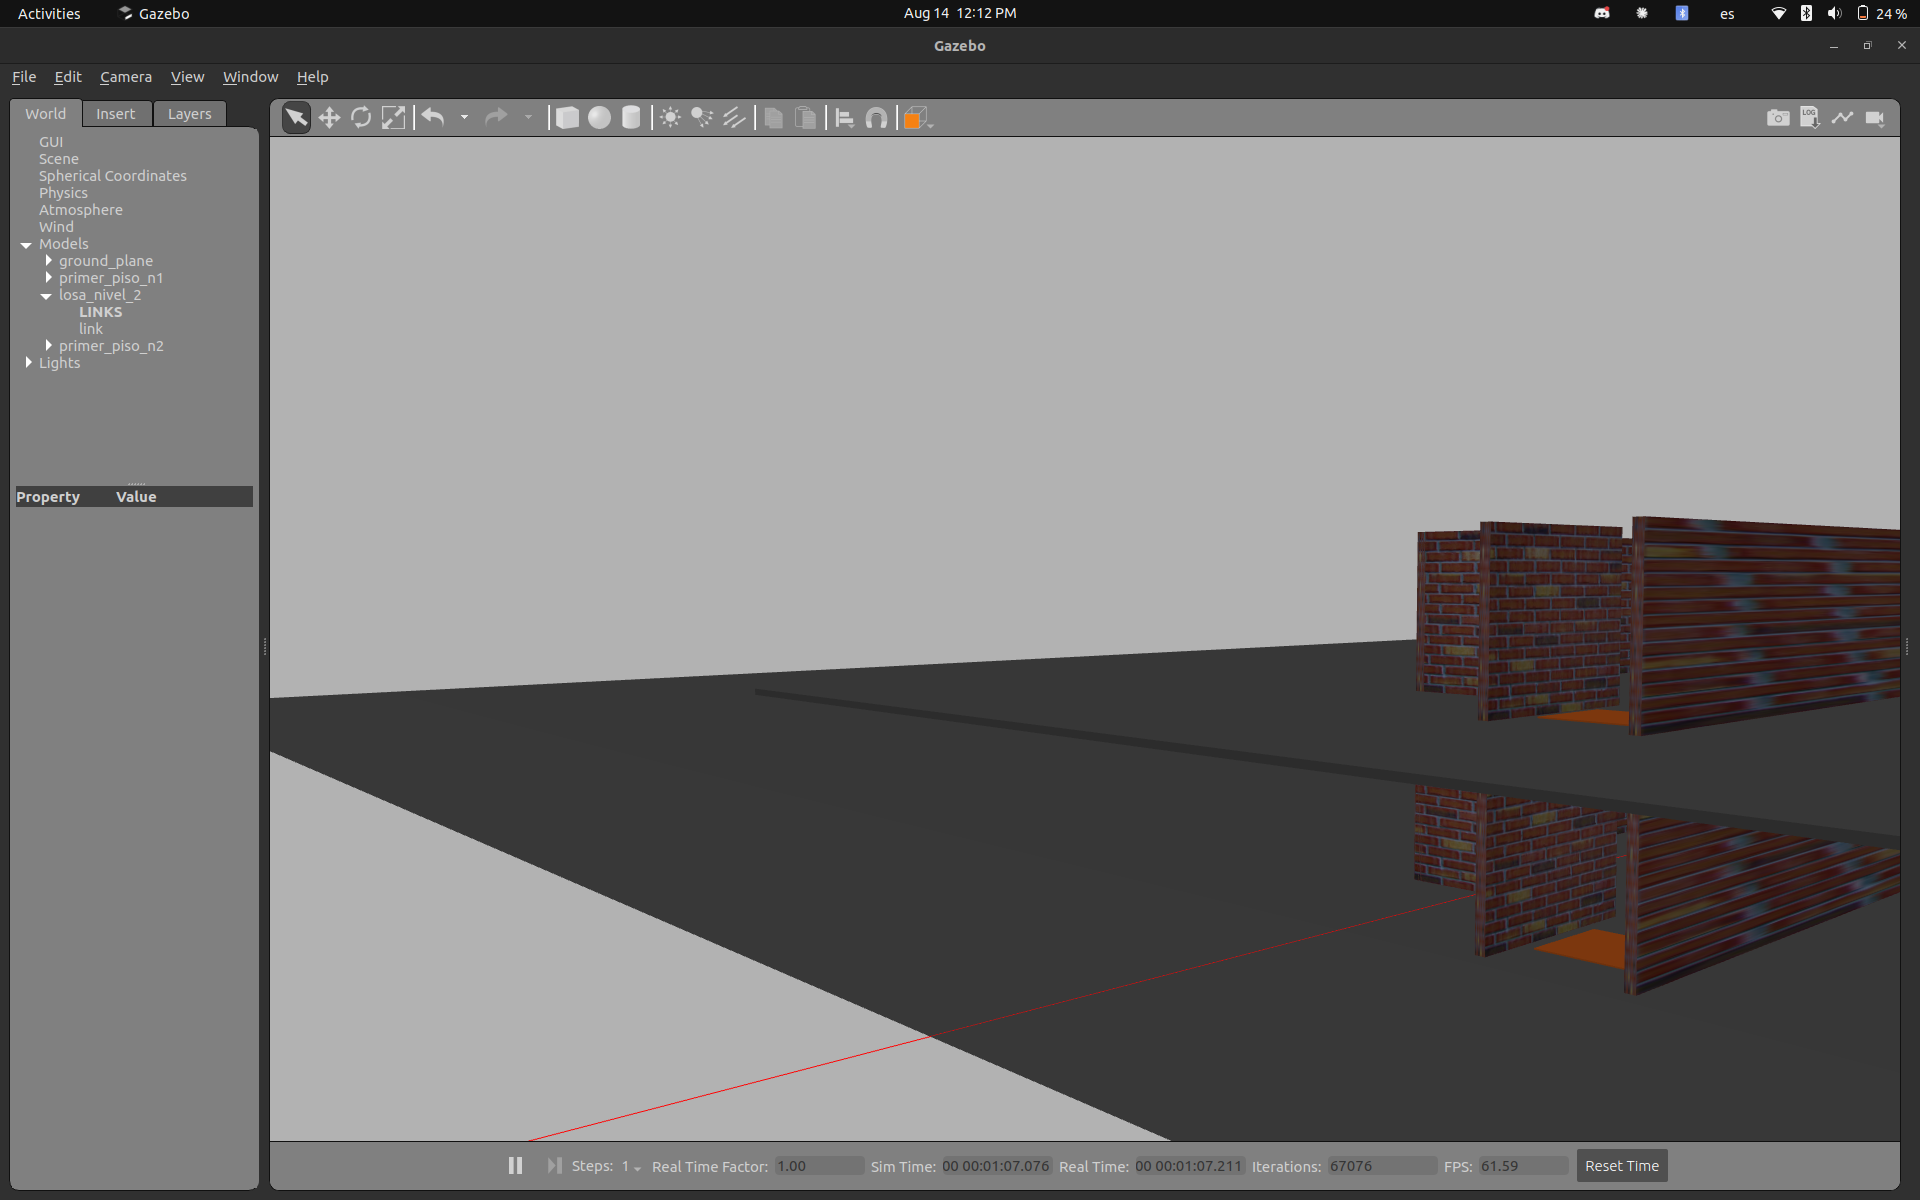
\includegraphics[width=0.95\textwidth]{S18_gazebo_dos_niveles.png}
    \caption{Entorno de evaluación con las dos plantas instanciadas y la zona de transición señalizada en cada nivel.}
    \label{fig:dos_niveles}
\end{figure}

\subsection{Zona de transición}

Se incorporó una marca de $1{,}5 \times 1{,}5$~m dentro del propio modelo de la planta, de modo que aparezca en las mismas coordenadas horizontales en los dos niveles. Se declara \textbf{sin volumen de colisión}: es una señal para el protocolo de relevo, no un obstáculo.

Sus coordenadas se derivaron de la geometría del edificio y no se eligieron por conveniencia. Se deja constancia de un hecho que refuerza la validez del entorno: al contrastarlas posteriormente con la planta real, el recinto obtenido por derivación geométrica \textbf{resultó ser el descanso de la escalera real}, sin que la planta se hubiera consultado durante la derivación.

\subsection{Navegación autónoma en el nivel superior}

Se comandó al vehículo un objetivo de navegación situado a 5,0 m en el nivel superior. Los resultados se presentan en la Tabla \ref{tab:nivel2}.

\begin{table}[H]
    \centering
    \small
    \caption{Navegación autónoma en el nivel superior, medida contra la odometría del simulador.}
    \label{tab:nivel2}
    \begin{tabular}{@{}lccc@{}}
        \toprule
        \textbf{Instante} & \textbf{Eje longitudinal} & \textbf{Eje transversal} & \textbf{Altura} \\ \midrule
        Antes del objetivo   & $-0{,}00095$ m & $-0{,}00977$ m & 2,9929972 m \\
        Después del objetivo & 4,78854 m & 0,07895 m & 2,9929953 m \\ \addlinespace
        Variación & \textbf{4,78949 m} & 0,08872 m & \textbf{1,9 micrómetros} \\ \bottomrule
    \end{tabular}
\end{table}

El recorrido real fue de \textbf{4,79 m} sobre un objetivo de 5,0 m, cifra equivalente a los 4,89 m y 4,96 m medidos sobre el mismo objetivo en el nivel inferior. El nivel superior se comporta igual que el inferior.

\textbf{La columna determinante es la altura}, que varió 1,9 micrómetros a lo largo de toda la corrida. Esta medición era necesaria y no redundante: las dos plantas son idénticas, de modo que \textbf{el LiDAR no puede distinguirlas}. Un vehículo que hubiese caído al nivel inferior produciría exactamente las mismas lecturas de rango, y tanto la localización como el planificador lo darían por correcto. Únicamente la altura discrimina entre ambos casos.

\subsection{Supresión de la actividad de mapeo del nivel superior}

La planificación de la semana contemplaba levantar un mapa propio del nivel superior. \textbf{Esta actividad se suprime}, y no por falta de tiempo.

El nivel superior es la misma planta en las mismas coordenadas horizontales. Un mapa de ocupación bidimensional es un \emph{corte horizontal} del entorno, de modo que el corte tomado a 0,30 m y el tomado a 3,30 m describen la misma geometría. Se comprobó con herramienta y no por argumento: ambos cortes producen mapas \textbf{idénticos píxel a píxel} entre sí y respecto del mapa vigente, y ambos superan la verificación automática del proyecto con 99,7 \% de cobertura y cero obstáculos sin pared real detrás.

Levantar un segundo mapa de la misma geometría solo podría introducir divergencias respecto del primero. La supresión es válida mientras las dos plantas sean idénticas, que es el caso real del edificio; queda registrada como condición.

Durante esta comprobación se detectó y corrigió un defecto en la herramienta generadora de mapas, expuesto en la Sección \ref{sec:corte}.

\section{Corrección del mapa de navegación}
\label{sec:mapa}

\subsection{Defecto detectado}

Se sometió el mapa de navegación en uso a la verificación automática del proyecto, contrastándolo contra la geometría del archivo de mundo. El resultado fue el rechazo del mapa: cobertura del 35,5 \% en el eje longitudinal frente a un mínimo exigido del 85 \%, una extensión transversal de 15,0 m frente a los 5,3 m reales del pasillo, y un 62,8 \% de celdas de estado desconocido.

El hallazgo determinante fue que \textbf{2688 de 3618 celdas marcadas como ocupadas, es decir el 74 \%, no tenían ninguna pared real detrás}. Eran paredes que el algoritmo de mapeo había construido a partir de su propia deriva de estimación.

La consecuencia no es estética. El planificador trata las celdas ocupadas como espacio letal, de modo que la navegación se interrumpía con un error de posición inicial en espacio letal \textbf{en tramos del pasillo que están libres}. El defecto no es visible al inspeccionar el mapa; se manifiesta mucho después y bajo otra denominación.

\subsection{Corrección aplicada}

La corrección se resolvió por una vía distinta de la prevista. En lugar de repetir el mapeo con parámetros ajustados, se desarrolló una herramienta que \textbf{deriva el mapa de la geometría declarada en el archivo de mundo}. El fundamento es que en simulación la geometría del mundo es la verdad del entorno, y un mapa construido por SLAM solo puede aproximarse a ella.

\begin{table}[H]
    \centering
    \small
    \caption{Comparación entre el mapa anterior y el mapa derivado de la geometría.}
    \label{tab:mapas}
    \begin{tabular}{@{}lcc@{}}
        \toprule
        \textbf{Indicador} & \textbf{Mapa por SLAM} & \textbf{Mapa derivado} \\ \midrule
        Cobertura longitudinal & 35,5 \% & \textbf{99,7 \%} \\
        Obstáculos sin pared real & 2688 de 3618 & \textbf{0 de 5149} \\
        Celdas de estado desconocido & 62,8 \% & 14,5 \% \\
        Deriva de localización medida & 0,323 m & \textbf{0,045 -- 0,100 m} \\ \bottomrule
    \end{tabular}
\end{table}

\subsection{Criterio derivado de este hallazgo}

Se adopta como norma del proyecto que \textbf{un resultado satisfactorio informado por la propia pila de navegación no constituye evidencia}. El controlador declara alcanzado un objetivo comparando contra la pose que le suministra el módulo de localización. Con el mapa defectuoso, la navegación informaba éxito sobre una pose que no era la real: el vehículo no había llegado y, en un caso, ni siquiera se había desplazado.

En consecuencia, toda medida de navegación del proyecto se contrasta contra la odometría que el complemento de tracción calcula a partir de la pose del cuerpo en el simulador. Es la única fuente que no depende de aquello que se está midiendo. Este criterio se aplica en las Tablas \ref{tab:navegacion} y \ref{tab:nivel2} de este informe.

\subsection{Un mapa bidimensional es un corte, no una proyección}
\label{sec:corte}

Al aplicar la herramienta generadora sobre el entorno de dos niveles se detectaron dos defectos encadenados. El primero es que solo interpretaba los modelos escritos en línea e ignoraba los incluidos por referencia, de modo que encontraba una pared en lugar de doce.

El segundo es conceptualmente más importante: la herramienta \textbf{proyectaba} toda la geometría sobre el plano en lugar de \textbf{cortarla} a una altura determinada. Mientras existió un solo nivel, ambas interpretaciones coincidían y la distinción no tenía costo. Con dos niveles, la losa del nivel superior ---una superficie de 50 por 20 m--- habría pintado el mapa completo como ocupado.

Se incorporó en consecuencia la altura de corte como parámetro explícito, tanto en el generador como en el verificador. Se comprobó que la corrección no altera el resultado sobre el entorno de un solo nivel: el archivo regenerado es idéntico byte a byte al versionado.

Se corrigió además un tercer defecto de la misma herramienta, que consideraba pared cualquier caja del modelo con independencia de si pertenecía a su volumen de colisión. Un elemento con representación visual y sin colisión ---exactamente el caso de la zona de transición--- habría aparecido como obstáculo. Un obstáculo inexistente en el mapa no produce ningún error: la localización converge igual y el planificador acepta objetivos igual; el síntoma aparece después, como una trayectoria que rodea algo que no existe.

\section{Reproducibilidad del entorno de desarrollo}

El repositorio del proyecto debe poder instalarse en un equipo distinto del de sus autores, dado que los directores requieren una versión ejecutable y que el propio proyecto se despliega sobre dos unidades de cómputo adicionales. Se incorporaron dos instrumentos de verificación automática:

\begin{table}[H]
    \centering
    \small
    \caption{Instrumentos de verificación del repositorio.}
    \label{tab:verificadores}
    \begin{tabular}{@{}p{4.6cm}p{4.3cm}p{4.4cm}@{}}
        \toprule
        \textbf{Instrumento} & \textbf{Pregunta que responde} & \textbf{Resultado} \\ \midrule
        Verificación de instalación & ¿El código compila y funciona en este equipo? & 31 comprobaciones, 0 fallos \\ \addlinespace
        Verificación documental & ¿Los documentos afirman lo que los artefactos sostienen? & 11 comprobaciones, 0 fallos \\ \bottomrule
    \end{tabular}
\end{table}

El segundo instrumento existe porque el primero no cubría nada de lo escrito: se disponía de treinta comprobaciones sobre el código y de ninguna sobre la documentación, lo cual explica que el código convergiera mientras los documentos divergían. Verifica la ausencia de rutas específicas de una máquina concreta, la existencia de los archivos citados, la validez de los enlaces y la coherencia entre lo que los documentos declaran y lo que el código ejecuta.

Se corrigieron los defectos que estos instrumentos revelaron. El de mayor consecuencia práctica: la ruta de búsqueda de modelos del simulador se deducía de una ubicación fija en lugar de la ubicación real de los archivos. En un equipo que hubiese clonado el repositorio en otro directorio, \textbf{el simulador abría un mundo vacío sin emitir error alguno}; y si existía otra copia en la ruta supuesta, se cargaba en silencio la geometría del repositorio equivocado. El caso se materializó durante la propia verificación.

La versión verificada se publicó etiquetada, de modo que exista un punto reproducible al cual referirse. Se comprobó desde un clon limpio: resolución de dependencias sin faltantes, compilación satisfactoria de los seis paquetes y ambos verificadores sin fallos.

\section{Hallazgos abiertos que condicionan el objetivo específico 4}
\label{sec:abiertos}

Se documentan tres hallazgos que permanecen abiertos. Ninguno afecta a la validez de los hitos cerrados esta semana; los tres son condiciones previas para instrumentar las métricas del objetivo específico 4, cuya totalidad se calcula sobre odometría.

\begin{table}[H]
    \centering
    \small
    \caption{Hallazgos abiertos y su efecto sobre el trabajo previsto.}
    \label{tab:abiertos}
    \begin{tabular}{@{}p{4.5cm}p{4.5cm}p{4.3cm}@{}}
        \toprule
        \textbf{Hallazgo} & \textbf{Descripción} & \textbf{Efecto} \\ \midrule
        Lectura de odometría cruzada & Una lectura informó 4,51 m de avance de un vehículo que permanecía inmóvil. Lo leído era la posición del otro vehículo, desplazada su distancia de aparición & Debe establecerse la causa antes de instrumentar métrica alguna. Medida provisional: leer sin el servicio de descubrimiento intermedio \\ \addlinespace
        Desviación con comando puramente lineal & Bajo un comando sin componente angular se midieron desviaciones de $9{,}5^\circ$, $15^\circ$ y aproximadamente $18^\circ$ en distintas corridas & Falsea cualquier medida de trayectoria. Sin causa determinada \\ \addlinespace
        Competencia en la carga de controladores & Un controlador puede quedar sin configurar de forma intermitente durante el arranque, dejando una rueda motriz sin actuar & Debe resolverse antes de tomar medidas de tiempo, porque altera la dinámica del vehículo \\ \bottomrule
    \end{tabular}
\end{table}

Los tres se atienden en la Semana 19, con anterioridad a cualquier instrumentación. Se considera preferible resolverlos antes que obtener mediciones que después habría que descartar, criterio que este mismo informe ha ilustrado en la Sección \ref{sec:mapa}.

\section{Aporte de la semana a los objetivos específicos}
\label{sec:aporte}

\subsection{Relación entre actividades y objetivos}

\begin{table}[H]
    \centering
    \small
    \caption{Trazabilidad entre las actividades ejecutadas y los objetivos específicos.}
    \label{tab:trazabilidad}
    \begin{tabular}{@{}p{4.0cm}cp{7.6cm}@{}}
        \toprule
        \textbf{Actividad} & \textbf{Objetivo} & \textbf{Contribución} \\ \midrule
        Dos agentes aislados bajo espacio de nombres (H1) & OE1, OE2 & Sin dos agentes direccionables por separado no existe destinatario al que asignar una tarea. Es la precondición de la asignación de tareas de OE1 y del componente de comunicación de OE2 \\ \addlinespace
        Entorno de dos niveles (H2b) & OE1, OE4 & Cubre el componente de escenarios multipiso de OE1 y convierte la continuidad entre niveles de OE4 en una magnitud medible \\ \addlinespace
        Corrección del mapa de navegación & OE4 & Cualquier métrica obtenida sobre el mapa anterior habría sido rebatible. La corrección es condición de validez de la campaña experimental completa \\ \addlinespace
        Criterio de medición contra odometría & OE4 & Establece qué se acepta como evidencia de desplazamiento, con anterioridad a instrumentar \\ \addlinespace
        Verificación de instalación y publicación etiquetada & Transversal & Permite que el sistema se despliegue sobre las dos unidades de cómputo del proyecto y que los directores dispongan de una versión ejecutable \\ \bottomrule
    \end{tabular}
\end{table}

\subsection{Estado de los objetivos específicos}

\begin{table}[H]
    \centering
    \small
    \caption{Avance por objetivo específico al cierre de la Semana 18.}
    \label{tab:objetivos}
    \begin{tabular}{@{}cp{2.0cm}p{4.4cm}p{5.2cm}@{}}
        \toprule
        \textbf{ID} & \textbf{Avance} & \textbf{Cubierto esta semana} & \textbf{Componente que lo mantiene detenido} \\ \midrule
        OE1 & 40 \% & Escenarios multipiso; base de la asignación de tareas & Matriz de requisitos funcionales y su trazabilidad a pruebas \\ \addlinespace
        OE2 & 40 \% & Comunicación entre agentes en simulación & Sensado con LiDAR físico y control desde ROS 2 sobre el vehículo real \\ \addlinespace
        OE3 & 0 \%  & --- & Programado para la Semana 22 \\ \addlinespace
        OE4 & 0 \%  & Condiciones de medida: entorno con dos niveles, mapa válido, criterio de evidencia & Instrumentación y protocolo experimental \\ \bottomrule
    \end{tabular}
\end{table}

\textbf{Los porcentajes no se desplazaron y conviene explicar por qué.} El indicador de avance se define sobre producto entregado, no sobre trabajo ejecutado. La Semana 18 produjo habilitadores: componentes cuyo valor no reside en avance propio sino en el trabajo que desbloquean. Presentar un incremento porcentual por este trabajo sería inexacto.

Lo que sí avanzó, y es el indicador pertinente para esta semana, es el estado de los hitos y del camino crítico. De los nueve hitos del cronograma actualizado, dos quedaron cerrados esta semana, y son los dos que bloqueaban al resto.

\subsection{Cadena de dependencia hacia el objetivo específico 4}

La siguiente cadena hace explícito por qué el trabajo de esta semana es condición del aporte declarado del proyecto. Cada eslabón bloquea al siguiente.

\begin{table}[H]
    \centering
    \small
    \caption{Cadena de dependencia desde los hitos de la Semana 18 hasta la evaluación.}
    \label{tab:cadena}
    \begin{tabular}{@{}clp{6.6cm}c@{}}
        \toprule
        \textbf{\#} & \textbf{Eslabón} & \textbf{Qué habilita} & \textbf{Estado} \\ \midrule
        1 & Contrato de interfaces (H1) & Que el coordinador mande a un agente sin conocer si es simulado o físico & Cerrado \\ \addlinespace
        2 & Dos agentes aislados (H1) & Que exista un destinatario distinguible al que asignar tarea & Cerrado \\ \addlinespace
        3 & Entorno de dos niveles (H2b) & Que la continuidad entre niveles sea medible & Cerrado \\ \addlinespace
        4 & Mapa válido & Que las métricas obtenidas sean defendibles & Cerrado \\ \addlinespace
        5 & Nodo de coordinación (S20) & Asignación dinámica de tareas por nivel & Pendiente \\ \addlinespace
        6 & Protocolo de relevo (S21) & El aporte técnico declarado del proyecto & Pendiente \\ \addlinespace
        7 & Instrumentación (S20--S21) & Registro automático de las cuatro métricas & Pendiente \\ \addlinespace
        8 & Campaña experimental (S24--S25) & Evidencia estadística de OE4 & Pendiente \\ \bottomrule
    \end{tabular}
\end{table}

Los cuatro primeros eslabones están cerrados. Los cuatro restantes constituyen el trabajo de las Semanas 20 a 25 y se encuentran, a partir de esta semana, sin dependencias previas sin resolver.

\section{Estado del cronograma y trabajo previsto}
\label{sec:cronograma}

\subsection{Cumplimiento del criterio de cierre}

El criterio de cierre establecido para la Semana 18 comprendía tres condiciones. Se cumplieron dos.

\begin{table}[H]
    \centering
    \small
    \caption{Criterio de cierre de la Semana 18.}
    \label{tab:cierre}
    \begin{tabular}{@{}p{8.5cm}p{5.0cm}@{}}
        \toprule
        \textbf{Condición} & \textbf{Resultado} \\ \midrule
        El hito H1 queda cerrado & Cumplido \\
        El entorno de dos niveles carga y se navega sobre él & Cumplido, con medición \\
        El diagnóstico de hardware responde sus cuatro preguntas & \textbf{No ejecutado} \\ \bottomrule
    \end{tabular}
\end{table}

El diagnóstico de hardware y la matriz de requisitos se trasladan a la Semana 19. La causa es que el cierre del hito H1 requirió más trabajo del previsto, al aparecer durante su ejecución tres defectos no contemplados: la imposibilidad de aislar dos vehículos en un mismo simulador, las referencias malformadas a los modelos geométricos, y el estado del mapa de navegación.

\subsection{Estado de actividades del anteproyecto}

\begin{table}[H]
    \centering
    \small
    \caption{Estado de actividades --- Semana 18 (Fase 5).}
    \label{tab:estado_s18}
    \begin{tabular}{@{}p{6.3cm}ll@{}}
        \toprule
        \textbf{Actividad (anteproyecto)} & \textbf{Estado} & \textbf{Observación} \\ \midrule
        Ajuste progresivo de los elementos desarrollados & Concluida & Cierre del hito H1 \\ \addlinespace
        Integración de los módulos del sistema & En curso & Dos agentes integrados; falta el coordinador \\ \addlinespace
        Análisis del entorno de evaluación & Concluida & Entorno de dos niveles construido y navegado \\ \addlinespace
        Registro de avances del proyecto & En curso & Presente entregable \\ \bottomrule
    \end{tabular}
\end{table}

\subsection{Constancia de revisión de los directores}

El documento \textit{Actividad 1 --- Corte 1}, que contiene el cronograma actualizado, la matriz de objetivos y evidencia, los hitos y la tabla de desviaciones, cuenta con constancia de revisión firmada dentro del plazo establecido.

Se deja constancia de dos precisiones sobre su alcance, en atención a la exactitud del registro:

\begin{itemize}
    \item La constancia recoge la revisión de \textbf{un} director. No debe citarse como aprobación de los tres.
    \item El documento revisado tiene fecha de corte anterior en un día a la adopción del entorno de dos niveles. En consecuencia, su actividad de modelado del entorno y su matriz de objetivos y evidencia todavía refieren el laboratorio como escenario de evaluación. \textbf{Esa referencia quedó superada por las decisiones de alcance revisadas}, según se expone en la Sección \ref{sec:desviacion}.
\end{itemize}

\subsection{Evolución de la decisión sobre el entorno de evaluación}
\label{sec:desviacion}

Se registra una decisión técnica que evolucionó durante el desarrollo y que difiere de lo consignado en el documento revisado. No se modifica el documento entregado; la divergencia se declara aquí y se comunicará en el próximo corte.

La planificación establecía como entorno de evaluación una réplica del laboratorio del grupo de investigación. El análisis del entorno concluyó que \textbf{el laboratorio no admite la pregunta de investigación}: son 16 m\textsuperscript{2} en un solo nivel, sin discontinuidad vertical, cuando la variable de respuesta principal es la continuidad del servicio entre niveles. Adicionalmente, el vehículo posee un círculo de giro de 0,57 m de diámetro, con lo cual los recorridos disponibles se reducen a dos o tres metros, y una sala cuadrada desprovista de mobiliario constituye el peor caso para la localización, dado que el sensor observa los cuatro muros desde cualquier posición.

El entorno adoptado es la planta real del primer piso del edificio, instanciada en dos niveles. \textbf{Esta réplica no constituye una simplificación de modelado sino la geometría real}: el segundo piso del edificio es idéntico al primero. El laboratorio conserva su función dentro del proyecto como \textbf{etapa de validación del hardware}, previa a las pruebas en el pasillo real.

El producto verificable resultante es más exigente que el planificado: el entorno pasó de un nivel a dos niveles con separación vertical real. Se considera, por tanto, una precisión del alcance derivada del análisis y no un incumplimiento.

\subsection{Trabajo previsto para la Semana 19}

La Semana 19 dispone de cuatro días hábiles. Las actividades previstas son:

\begin{itemize}
    \item \textbf{Matriz de requisitos funcionales}, con su trazabilidad a objetivos específicos y a pruebas de verificación. Es el artefacto que mantiene detenido el objetivo específico 1 y el que hace posible la comparación con requisitos que el anteproyecto exige.
    \item \textbf{Diagnóstico de hardware}, reordenado. Tres de sus cuatro preguntas se resuelven con un solo vehículo; la relativa a la latencia de comunicación requiere ambos y queda supeditada a la finalización de la intervención técnica que uno de ellos se encuentra atravesando. Se antepone la pregunta relativa a la diferencia entre distribuciones de ROS 2, que no requiere hardware encendido.
    \item \textbf{Protocolo experimental del objetivo específico 4}: qué se mide, mediante qué procedimiento, con cuántas repeticiones y bajo qué criterio de éxito. Se redacta \emph{antes} de instrumentar.
    \item \textbf{Resolución de los tres hallazgos abiertos} de la Sección \ref{sec:abiertos}.
    \item \textbf{Los dos agentes navegando de forma simultánea, cada uno en su nivel.} Por separado ya está demostrado; falta la corrida conjunta, que constituye el hito H3.
\end{itemize}

Se registra una diferencia entre las distribuciones de ROS 2 que ha adquirido relevancia: el entorno de simulación opera sobre la distribución Humble, mientras que las dos unidades de cómputo de los vehículos operan sobre Jazzy. La diferencia está confirmada y falta caracterizar su magnitud, tarea que afecta de forma directa al nodo de coordinación previsto para la Semana 20, el cual debe comunicarse con ambos vehículos.

\section{Conclusiones de la Semana}

Durante la Semana 18 quedaron cerrados los dos hitos que bloqueaban la totalidad del desarrollo posterior. El hito H1 se cerró con dos agentes robóticos ejecutando pilas de navegación completas de forma simultánea, cada uno bajo su propio espacio de nombres, con aislamiento de mando demostrado mediante cuatro evidencias independientes y con desplazamiento verificado contra la odometría del simulador. El hito H2b se cerró con un entorno de evaluación de dos niveles verticales reales, sobre cuyo nivel superior se navegó de forma autónoma con la altura constante a 1,9 micrómetros.

Se detectó y corrigió un defecto en el mapa de navegación cuya consecuencia no era estética: el 74 \% de sus celdas ocupadas no correspondía a ninguna pared real, lo que interrumpía la planificación en tramos libres del pasillo. La corrección se resolvió derivando el mapa de la geometría del entorno simulado, con lo cual la deriva de localización descendió de 0,323 m a un intervalo entre 0,045 m y 0,100 m. De este hallazgo se derivó un criterio metodológico que rige el resto del proyecto: un resultado satisfactorio informado por la propia pila de navegación no constituye evidencia.

Una actividad planificada quedó suprimida por comprobación y no por falta de tiempo: el levantamiento de un mapa propio del nivel superior. Un mapa de ocupación bidimensional es un corte horizontal, de modo que los cortes de ambos niveles resultan idénticos píxel a píxel.

El diagnóstico de hardware y la matriz de requisitos no se ejecutaron y se trasladan a la Semana 19. Se declara de forma explícita: de las tres condiciones del criterio de cierre de la semana, se cumplieron dos.

El balance de la semana no se expresa en avance porcentual de los objetivos específicos, que permanecen en sus valores previos, sino en el estado del camino crítico. Los cuatro primeros eslabones de la cadena que conduce a la evaluación del objetivo específico 4 están cerrados, y los cuatro restantes se encuentran, por primera vez, sin dependencias previas sin resolver.

\begin{thebibliography}{99}

\bibitem{entregable17}
S. Hernández Ávila y J. A. Mejía León,
``Informe de Avance --- Semana 17,''
Universidad Santo Tomás, Facultad de Ingeniería Electrónica, Bogotá, agosto de 2026.

\bibitem{cronograma}
S. Hernández Ávila y J. A. Mejía León,
``Cronograma de actividades --- Semanas 17 a 32,''
Universidad Santo Tomás, Facultad de Ingeniería Electrónica, Bogotá, agosto de 2026.

\bibitem{anteproyecto}
S. Hernández Ávila y J. A. Mejía León,
``Sistema colaborativo de robots móviles para asistencia de orientación en entornos interiores con múltiples pisos --- Anteproyecto,''
Universidad Santo Tomás, Facultad de Ingeniería Electrónica, Bogotá, 2026.

\bibitem{ros2_humble_docs}
Open Robotics,
``ROS 2 Humble Hawksbill Documentation,''
[Online]. Available: \url{https://docs.ros.org/en/humble/}

\bibitem{nav2_docs}
Open Robotics,
``Nav2 Documentation,''
[Online]. Available: \url{https://docs.nav2.org/}

\bibitem{gazebo}
Open Robotics,
``Gazebo Classic Documentation,''
[Online]. Available: \url{https://classic.gazebosim.org/tutorials}

\bibitem{tf2}
Open Robotics,
``tf2: The transform library,''
[Online]. Available: \url{https://docs.ros.org/en/humble/Concepts/Intermediate/About-Tf2.html}

\bibitem{slam_toolbox}
S. Macenski and I. Jambrecic,
``SLAM Toolbox: SLAM for the dynamic world,''
Journal of Open Source Software, vol. 6, no. 61, p. 2783, 2021. [Online]. Available: \url{https://github.com/SteveMacenski/slam_toolbox}

\end{thebibliography}

\end{document}
